\newpage
{\bfseries IRSTI 61.31.57}
\hfill {\bfseries \href{https://doi.org/10.58805/kazutb.v.2.23-459}{https://doi.org/10.58805/kazutb.v.2.23-459}}

\sectionwithauthors{M.K. Kazankapova, B.T. Yermagambet, Zh.T. Dauletzhanova, A.M. Kalenova}{OBTAINING POROUS CARBON MATERIAL AND INVESTIGATION OF ITS PHYSICAL AND CHEMICAL PROPERTIES}

\begin{center}
{\bfseries \textsuperscript{1,2}M.K. Kazankapova, \textsuperscript{1}B.T. Yermagambet, \textsuperscript{1,2}Zh.T. Dauletzhanova\envelope, \textsuperscript{1}A.M. Kalenova}

\textsuperscript{1}LLP "Institute of Coal Chemistry and Technology",
Astana, Kazakhstan,

\textsuperscript{2}Kazakh University of Technology and Business named
after K. Kulazhanov, Astana

\envelope Corresponding author: kaliyeva\_zhanna@mail.ru
\end{center}

The work carried out a physicochemical analysis of porous carbon
material (PCM) obtained from brown coal from the Maikuben basin
(Kazakhstan). PUM was obtained by carbonization and activation in argon
and water vapor. The electrophysical characteristics of the PCM were
determined by measuring the electrical capacitance of the samples in the
temperature range 293−483 K. The resulting product exhibits high
characteristics, including high dielectric permittivity, specific
surface area, and capacity, making it effective for use in
supercapacitors as an electrode material and for hydrogen storage. The
coal carbonization process includes an initial low-temperature (at
180°C, with a heating rate of 10°C/min) treatment of the raw material in
the presence of air for 1 hour, followed by carbonization in an inert
atmosphere at temperatures ranging from 180-900°C with a heating rate of
5°C/min, and steam activation at the maximum temperature for 1 hour of
the coal ground to a 0.1 mm fraction. The material is then extruded into
cylindrical shapes (diameter: 2-3 mm, length: 5-10 mm) using a binder
material: starch - 5\%, sodium hydroxide - 0.5\%, water - 17\% of the
total mass of coal.

{\bfseries Keywords:} porous carbon material (PCM), brown coal,
carbonization, activation, thermal decomposition, activated carbon.

\begin{center}
{\large\bfseries КЕУЕКТІ-КӨМІРТЕКТІ МАТЕРИАЛДЫ АЛУ ЖӘНЕ ОНЫҢ ФИЗИКАЛЫҚ-ХИМИЯЛЫҚ
ҚАСИЕТТЕРІН ЗЕРТТЕУ}

{\bfseries \textsuperscript{1,2}М.К. Казанкапова, \textsuperscript{1}Б.Т. Ермағамбет, \textsuperscript{1,2}Ж.Т. Даулетжанова\envelope, \textsuperscript{1}А.М. Каленова}

\textsuperscript{1}«Көмір химиясы және технологиясы институты» ЖШС,
Астана, Қазақстан,

\textsuperscript{2}Қ.Құлажанов атындағы Қазақ технология және бизнес
университеті, Астана, Қазақстан,

e-mail: coaltech@bk.ru
\end{center}

Жұмыс барысында Майкөбен бассейнінің (Қазақстан) қоңыр көмірінен алынған
кеуекті көміртекті материалға (ККМ) физика-химиялық талдау жүргізілді.
ККМ аргон мен су буында карбонизация және активтену арқылы алынды. ККМ
электрофизикалық сипаттамалары 293−483 К температура диапазонында
үлгілердің электр сыйымдылығын өлшеу арқылы анықталды. Алынған өнімнің
жоғары сипаттамалары бар, оның ішінде жоғары диэлектрлік өтімділігі,
меншікті бетінің ауданы және сыйымдылығы бар, бұл оны
суперконденсаторларда электрод материалы ретінде пайдалану үшін,
сондай-ақ сутегі сақтау үшін тиімді етеді. Көмірді карбонизациялау
процесі шикізатты 1 сағат бойы ауа қатысында төмен температурада (180°С,
қыздыру жылдамдығы 10°С/мин), содан кейін температура диапазонында
инертті ортада көміртектеуді қамтиды. 180-900°С қыздыру жылдамдығы
5°С/мин және су буымен 1 сағат максималды температурада белсендіріледі,
көмірдің 0,1 мм фракциясына дейін ұсақталады, содан кейін цилиндрлік
пішіндерге экструдталған (диаметрі 2-3 мм, ұзындығы 5-10 мм)
байланыстырушы материалды пайдалана отырып: крахмал -- 5\%, натрий
гидроксиді -- 0,5\%, су -- 17\% көмірдің жалпы массасынан.

{\bfseries Түйін сөздер:} кеуекті көміртекті материал (ПКМ), қоңыр көмір,
көміртендіру, активтену, термиялық ыдырау, белсендірілген көмір.
\newpage
\begin{center}
{\large\bfseries ПОЛУЧЕНИЕ ПОРИСТО-УГЛЕРОДНОГО МАТЕРИАЛА И ИССЛЕДОВАНИЕ ЕГО
ФИЗИКО-ХИМИЧЕСКИХ СВОЙСТВ}

{\bfseries \textsuperscript{1,2}М.К. Казанкапова, \textsuperscript{1}Б.Т.
Ермагамбет, \textsuperscript{1,2}Ж.Т. Даулетжанова\envelope,
\textsuperscript{1}А. М.Каленова,}

\textsuperscript{1}ТОО «Институт Химии угля и технолоогии, Астана,
Қазақстан,

\textsuperscript{2}Казахский университет технологии и бизнеса имени К.
Кулажанова, Астана, Казахстан,

e-mail: coaltech@bk.ru
\end{center}

В работе проведен физико-химический анализ пористо-углеродного материала
(ПУМ) полученного на основе бурого угля Майкубенского бассейна
(Казахстан). ПУМ получен методом карбонизации и активации в средах
аргона и водяного пара. Определены электрофизические характеристики ПУМ
путем измерения электроемкости образцов в интервале температур 293−483
К. Полученный продукт имеет высокие характеристики, включая высокую
диэлектрическую проницаемость, удельную поверхность и емкость, что
делает его эффективным для использования в суперконденсаторах в качестве
электродного материала, также для хранения водорода. Процесс
карбонизации угля, включал предварительную низкотемпературную (при
180°С, со скоростью нагрева 10°С/мин) обработку сырья в присутствии
воздуха в течение 1 часа, затем карбонизацию в инертной среде в
интервале температур 180-900°С со скоростью нагрева 5°С/мин и активацией
водяным паром при максимальной температуре в течение 1 часа измельченной
до фракции 0,1 мм угля, а затем экструдированием в цилиндрические формы
(диаметр-2-3 мм, длина 5-10 мм) с применением связующего материала:
крахмал - 5 \%, гидроксид натрия -- 0,5 \%, вода -- 17 \% от общей массы
угля.

{\bfseries Ключевые слова:} пористо-углеродный материал (ПУМ), бурый уголь,
карбонизация, активация, термическое разложение, активированный уголь.

\begin{multicols}{2}
{\bfseries Introduction}. Porous carbon nanomaterials, such as biochar,
graphene, and carbon nanotubes, have a wide range of applications in
heavy metal adsorption, energy storage, and sensor technologies due to
their excellent properties, such as high specific surface area (SSA) and
high electrical conductivity. Various synthesis methods for porous
carbon materials have been developed using a broad spectrum of raw
materials. For instance, chemical vapor deposition (CVD) is employed to
produce high-quality graphene from methane. However, these methods are
complex, and the raw materials used are either rare or expensive,
hindering the large-scale production and commercialization of advanced
carbon materials {[}1-5{]}.

Biomass is an exciting raw material for advanced porous carbon
nanomaterials through simple pyrolysis. Typically, the production of
porous carbon nanomaterials from biomass has two main advantages. First,
the cost of producing porous carbon nanomaterials can be significantly
lower. Biomass has diverse sources, ranging from straw, husks, leaves,
peels, to microorganisms and chitin, which are low-cost products of
agriculture, industry, and daily life. Second, it helps mitigate
environmental pollution caused by biomass. Biomass is usually discarded,
leading to environmental pollution, especially a large amount of carbon
dioxide (CO\textsubscript{2}) released into the atmosphere, exacerbating
the greenhouse effect. To address the issue of electromagnetic radiation
pollution, a simple method exists for producing porous carbon using coal
processing residues as a carbon source {[}6-14{]}.

The intensification of environmental issues, the need for comprehensive
wastewater treatment, gas emissions purification, and the disposal of
hazardous components necessitate the development of new methods and
approaches for creating industrial adsorbents {[}15{]}. This also
involves a more rational approach to the use of natural resources, the
application of hydrocarbon recovery processes, or the concentration of
rare metals from highly diluted solutions. One optimal solution to these
challenges may be the comprehensive use of high-quality and
cost-effective carbon adsorbents, such as activated carbons {[}16{]}.
Due to their physicochemical properties, carbon adsorbents are unique
and ideal sorption materials that can address a wide range of issues
related to ensuring chemical, biological, and radiation safety for
humans, the environment, and infrastructure. Among all available
adsorbents, activated carbons are the most versatile, capable of
absorbing a wide spectrum of toxicants {[}17-18{]}.

There are several methods for producing porous carbon material and
studying its physicochemical properties. One of the most common methods
is the thermal decomposition of organic substances (pyrolysis) in the
absence of oxygen (or at very low concentrations) followed by an
activation process, which involves treating the carbon structures with
chemical reagents or steam at high temperatures. This increases the
material\textquotesingle s porosity, forming micro-, meso-, and
macropores.

The obtained porous carbon material is subjected to various analytical
methods to study its physicochemical properties. This can include
measuring the porous structure (specific surface area, specific pore
volume, pore size distribution, sorption capacity, etc.), surface
chemical analysis (spectroscopy, chromatography), electrochemical
property studies, and other methods {[}19{]}.

Porous carbon materials can be applied in a wide range of fields,
including supercapacitors, catalysts, water purification, hydrogen
storage, and other areas {[}20{]}. Porous carbon materials (PCM) with a
high specific surface area (up to 1200 m²/g), open slit-type porosity,
high electrical conductivity, chemical stability, and low specific
weight have the potential to significantly improve the specific
characteristics of energy storage devices. PCMs based on coal can be
utilized in micro- and nanoelectronics, particularly as solid-state
electrode materials for supercapacitors, and can be used as energy
storage devices and power supplies for various high-power consumers that
have strict requirements for environmental friendliness, cyclic
resource, and readiness for operation, such as in electric vehicles,
solar panels, and satellites. These materials can store much more energy
than traditional capacitive elements, doing so for extended periods
without charge leakage {[}21{]}.

{\bfseries Materials and Methods.} There are numerous methods for producing
porous carbon materials from various carbon-containing substances. The
main difference between these methods is the aggressive reaction
environment required for the carbonization process, which necessitates
costs for washing and neutralizing the pH, as well as energy
expenditures for drying the products.

The proposed method involves the following stages: thermal treatment of
the raw material in an inert gas atmosphere up to 900ºC, followed by
activation of the carbon material.

The main advantages of this method are the use of readily available raw
materials, specifically brown coal from Kazakhstan (Maikuben basin,
Shoptykol deposit, W\_\textsuperscript{daf} -- 12.11\%,
A\_\textsuperscript{daf} -- 23.44\%, and V\_\textsuperscript{daf} --
40.66\%); the use of steam instead of caustic sodium for activation; the
production of a ready-to-use product through extrusion; and the
production of PCM with high dielectric permittivity (ε = 1.12×10⁹ at 483
K), a specific surface area of 348.99 m²/g, specific resistance of 3-4
ohms, and a capacitance of 1.2-1.7 µF.

The electrophysical properties (dielectric permittivity and electrical
resistance) of the obtained samples were measured using an LCR-800
series device (Taiwan) at a working frequency of 1 kHz in dry air under
a thermostat regime with a fixed temperature hold time. The Sawyer-Tower
circuit was used to obtain the relationship between electric induction
(D) and electric field strength (E). Visual observation of the D(E)
hysteresis loops was conducted on an S1-83 oscilloscope with a voltage
divider consisting of 6 MΩ and 700 kΩ resistors and a reference
capacitor of 0.15 µF. The generator frequency was 300 Hz. For all
temperature studies, the samples were placed in a furnace, and the
temperature was measured using a chromel-alumel thermocouple connected
to a V2-34 voltmeter with an error of ±0.1 mV. The temperature change
rate was approximately 5 K/min. The dielectric permittivity at each
temperature was determined using the formula ε = C/C₀, where C₀ is the
capacitance of the capacitor without the test substance (air).

The specific resistance and capacitance of the PCM were measured using a
digital multimeter "UT-70 B" (China).

The chemical analysis and surface morphology of the PCM were studied
using energy-dispersive X-ray spectroscopy (EDS) on a SEM (Quanta 3D
200i) equipped with an EDAX EDS attachment. The excitation electron beam
energy was 15 keV.

The phase composition of the PCM was identified using X-ray diffraction.
The X-ray phase analysis was conducted on a DRON-2 setup. Shooting
conditions: FeKα radiation, U = 28 kV, J = 28 mA.

The adsorption characteristics of the PCM (specific surface area) were
studied using the Brunauer-Emmett-Teller (BET) method. Measurements were
conducted on a KATAKON Sorbtometer M device.

\emph{Carbonization and Activation}

Carbonization and activation were carried out in a laboratory
high-temperature rotary furnace BR-12NRT (Figure 1).
\end{multicols}

\begin{figure}[H]
  \centering
  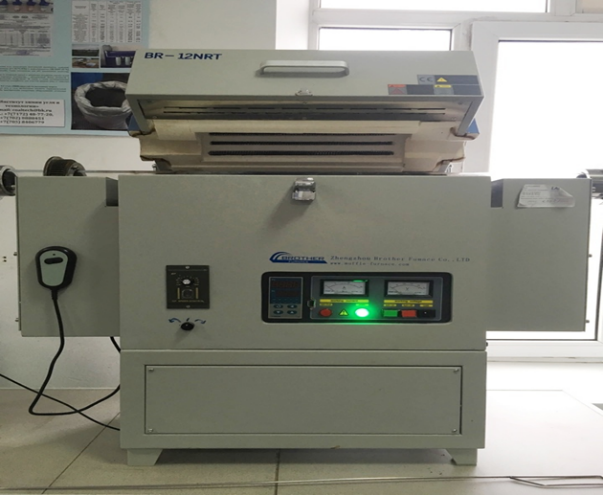
\includegraphics[width=0.5\textwidth]{assets/1089}
	\caption*{Fig. 1-High-Temperature Rotary Tube Furnace BR-12NRT}
\end{figure}

\begin{multicols}{2}
The coal underwent an initial low-temperature treatment (at 180°C, with
a heating rate of 10°C/min) in the presence of air for 1 hour, followed
by carbonization in an inert atmosphere at temperatures ranging from
180-900°C with a heating rate of 5°C/min, and steam activation at the
maximum temperature for 1 hour. The coal was ground to a 0.1 mm
fraction, extruded into cylindrical shapes (diameter: 2-3 mm, length:
5-10 mm) using a binder material: starch - 5\%, sodium hydroxide -
0.5\%, water - 17\% of the total mass of coal.

{\bfseries Results and Discussion}. The results of the elemental analysis
of the PCM obtained at 900°C, presented in Table 2, indicate that after
the thermal treatment of the coal, a significant portion of the volatile
components are removed as gaseous products, thereby increasing the
concentration of the mineral constituents.
\end{multicols}

\begin{table}[H]
\caption*{Table 1-Chemical Composition of PCM}
\centering
\begin{tabular}{|l|l|l|l|l|l|l|l|l|}
\hline
\textbf{Element} & \textbf{C} & \textbf{O} & \textbf{Mg} & \textbf{Al} & \textbf{Si} & \textbf{K} & \textbf{Ca} & \textbf{Fe} \\ \hline
Raw Coal, wt\% & 62.33 & 24.88 & 0.34 & 3.39 & 6.71 & 0.73 & 0.37 & 0.87 \\ \hline
PCM, wt\% & 60.69 & 19.44 & 0.58 & 5.29 & 10.09 & 01.05 & 0.75 & 1.60 \\ \hline
\end{tabular}
\end{table}

The X-ray phase analysis showed that the PCM is almost X-ray amorphous,
with weak reflections of SiO\textsubscript{2},
Fe\textsubscript{2}O\textsubscript{3}, and K\textsubscript{2}O observed.

Micrographs of the raw coal samples and the activated PCMs derived from
it are shown in Figure 2.

\begin{figure}[H]
    \centering
    \begin{subfigure}[b]{0.32\textwidth}
        \centering
        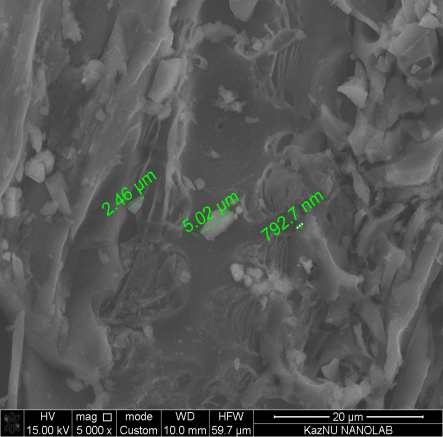
\includegraphics[height=4cm]{assets/1090}
        \caption*{×5000}
        \caption*{(а)}
    \end{subfigure}
    \hfill
    \begin{subfigure}[b]{0.32\textwidth}
        \centering
        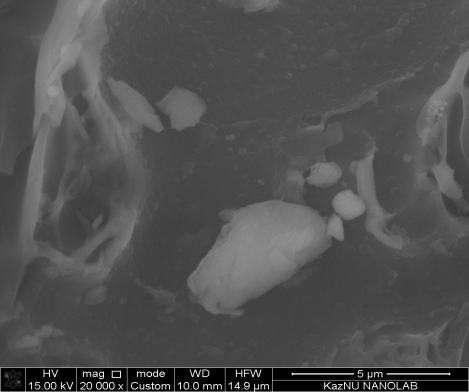
\includegraphics[height=4cm]{assets/1091}
        \caption*{×20000}
        \caption*{(b)}
    \end{subfigure}
    \hfill
    \begin{subfigure}[b]{0.32\textwidth}
        \centering
        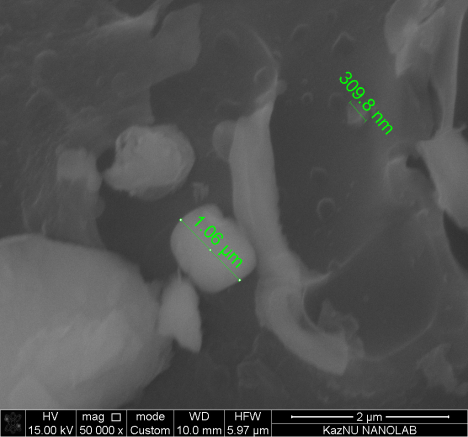
\includegraphics[height=4cm]{assets/1092}
        \caption*{×50000}
        \caption*{(c)}
    \end{subfigure}
\end{figure}

\begin{figure}[H]
    \centering
    \begin{subfigure}[b]{0.32\textwidth}
        \centering
        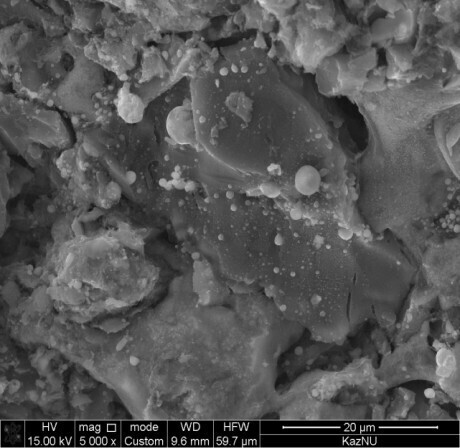
\includegraphics[height=4cm]{assets/1093}
        \caption*{×5000}
        \caption*{(d)}
    \end{subfigure}
    \hfill
    \begin{subfigure}[b]{0.32\textwidth}
        \centering
        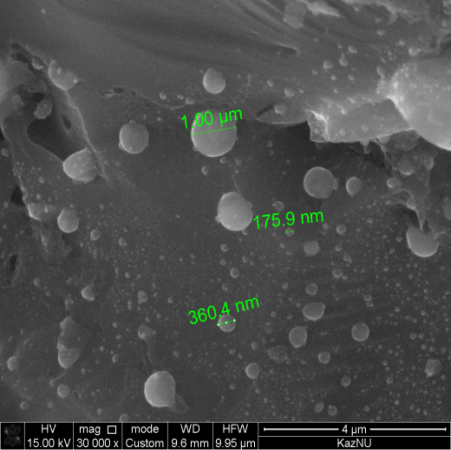
\includegraphics[height=4cm]{assets/1094}
        \caption*{×30000}
        \caption*{(f)}
    \end{subfigure}
    \hfill
    \begin{subfigure}[b]{0.32\textwidth}
        \centering
        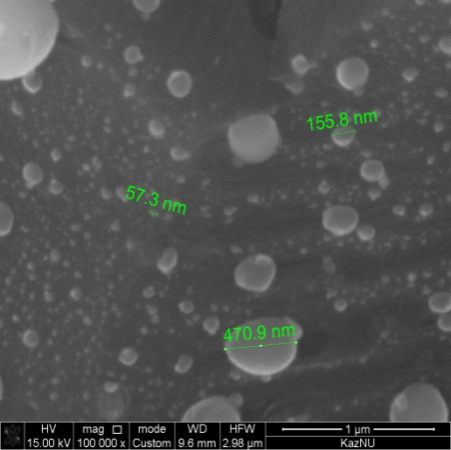
\includegraphics[height=4cm]{assets/1095}
        \caption*{×100000}
        \caption*{(g)}
    \end{subfigure}
    \caption*{Fig. 2 - Scanning Electron Microscope Images of Raw Coal (a) -- (c) and PCM (d) -- (g)}
\end{figure}

\begin{multicols}{2}
The analysis of the surface morphology of raw coal revealed a
heterogeneous structure characterized by flake-like inclusions in the
carbon matrix and particles with a plate-stepped shape. The SEM images
show that after thermal activation of the coal, the surface structure
becomes more developed with smaller particle sizes. The specific surface
area and specific pore volume significantly increase compared to the raw
sample-from 5.11 to 348.99 m²/g, approximately 70 times greater due to
high-temperature activation. The SEM images of the PCM show the
formation of fine nano- and macro-particles of silicon on the surface,
with diameters ranging from \textasciitilde50 nm to \textasciitilde1 μm.

The results of electrophysical studies show that PCM obtained at 300°C
exhibits metallic conductivity in the range of 293-373 K, semiconductor
conductivity at 373-413 K, metallic again at 413-443 K, and
semiconductor conductivity at 443-483 K. The bandgap width at 373-413 K
is 1.68 eV, and at 443-483 K, it is 2.24 eV, classifying the PCM as a
narrow-band semiconductor. The dielectric permittivity values are low,
with the specific surface area of the adsorbent being 7.51 m²/g. The
specific resistance of PCM is higher than MΩ, and the PCM does not
exhibit capacitance accumulation.

PCM obtained at 400°C shows metallic conductivity in the range of
293-333 K, semiconductor conductivity at 333-383 K, metallic again at
383-433 K, and semiconductor conductivity at 433-483 K. The bandgap
width at 333-383 K is 1.24 eV, and at 433-483 K, it is 1.84 eV,
classifying it as a narrow-band semiconductor. The dielectric
permittivity values are also low, with the specific surface area of the
adsorbent being 20.95 m²/g. The specific resistance of PCM is higher
than MΩ, and the PCM does not exhibit capacitance accumulation.

PCM obtained at 500°C shows semiconductor conductivity in the range of
293-353 K, metallic conductivity at 353-403 K, semiconductor again at
403-473 K, and metallic conductivity at 473-483 K. The bandgap width at
293-353 K is 0.79 eV, and at 403-473 K, it is 1.24 eV, classifying it as
a narrow-band semiconductor. The dielectric permittivity values are low,
with the specific surface area of the adsorbent being 161.42 m²/g. The
specific resistance of PCM is higher than MΩ, and the PCM does not
exhibit capacitance accumulation.

PCM obtained at 600°C shows semiconductor conductivity in the range of
293-343 K, metallic conductivity at 343-393 K, semiconductor again at
393-463 K, and metallic conductivity at 463-483 K. The bandgap width at
293-343 K is 0.87 eV, and at 393-463 K, it is 1.37 eV, classifying it as
a narrow-band semiconductor. The dielectric permittivity values are low,
with the specific surface area of the adsorbent being 150.98 m²/g. The
specific resistance of PCM is higher than MΩ, and the PCM does not
exhibit capacitance accumulation.

PCM obtained at 700°C exhibits semiconductor conductivity in the range
of 293-353 K, metallic conductivity at 353-363 K, and semiconductor
conductivity again at 363-483 K. The bandgap width of this adsorbent in
the range of 293-353 K is 0.75 eV, and at 363-483 K, ΔE = 0.86 eV,
classifying it as a narrow-band semiconductor. This adsorbent also
possesses giant dielectric permittivity values: 1.87·10⁷ at 293 K and
1.01·10⁹ at 463 K, making this material highly promising for
microcapacitor technology. The specific surface area of the adsorbent is
156.26 m²/g. The specific resistance of PCM is 280-600 Ω. The
capacitance of PCM is 0.01 μF.

PCM synthesized at 800°C shows metallic conductivity in the range of
293-313 K and semiconductor conductivity in the range of 313-483 K. The
bandgap width in the range of 313-483 K is 0.59 eV, classifying it as a
narrow-band semiconductor, with high dielectric permittivity values
increasing from 1.56·10⁷ (at 293 K) to 6.48·10⁸ (at 453 K). This
adsorbent is also of interest for microcapacitor technology. The
specific surface area of the adsorbent is 241.945 m²/g. The specific
resistance of PCM is 250-270 Ω. The capacitance of PCM is 0.58 μF.

PCM obtained at a higher temperature of 900°C exhibits semiconductor
properties in the range of 293-433 K, and metallic properties at 433-453
K. A second-order phase transition is observed at 433 K. This material
has significantly high dielectric permittivity values: \textasciitilde33
million at 293 K and over one billion (1.12·10⁹) at 483 K. The PCM
sample is of interest both as a semiconductor and as a promising
material for microcapacitor technology. The specific surface area of the
adsorbent is 348.99 m²/g. The specific resistance of PCM is 3-4 Ω. The
capacitance of PCM is 1.2-1.7 μF.

At high temperatures ranging from 700°C to 900°C, an increase in
dielectric permittivity (ε) is observed (Figure 3). The data shows that
PCM obtained at 900°C exhibits giant dielectric permittivity values,
reaching up to 1.12·10⁹ at 483 K, making it a highly promising material
for microcapacitor technology. The increase in dielectric permittivity
can be explained by the increase in the specific surface area of PCM, as
the specific capacitance of electrode materials is directly proportional
to the specific surface area. The increase in specific surface area is
due to the carbonization of the raw material in the temperature range of
700-900°C, where heteroatoms are removed, and the structure of flat
aromatic rings develops, forming basic structural units or elementary
graphite crystallites.
\end{multicols}

\begin{figure}[H]
  \centering
  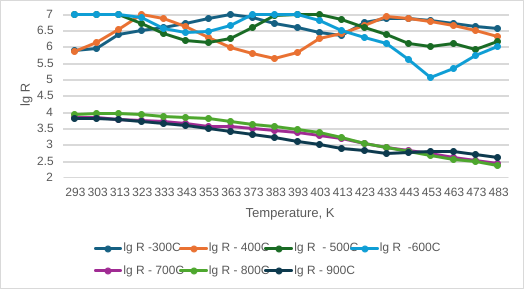
\includegraphics[width=0.56\textwidth]{assets/1098}
	\caption*{a}
\end{figure}

\begin{figure}[H]
  \centering
  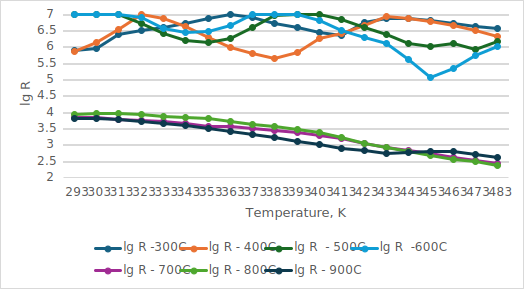
\includegraphics[width=0.56\textwidth]{assets/1097}
	\caption*{b}
	\caption*{Fig. 3 - Dependence of Electrical Resistance (R) and Dielectric Permittivity (ε) on Temperature for PCM Obtained at Different Temperature Intervals}
\end{figure}

\begin{multicols}{2}
Part of the carbon transitions from sp³ to sp² state, while some is
removed with gaseous and liquid components. Graphenes, consisting of
flat polycyclic aromatic molecules with two-dimensional ordering of
carbon atoms, form in the solid material volume. Steam activation
creates microporous structures by opening pores that are in a closed
state in the carbon material. Based on the analysis of the diagrams
constructed from the experimental data, the following conclusions can be
drawn:

Dielectric Permittivity (ε): an increase in the processing temperature
of coal leads to a significant increase in the dielectric permittivity
of the material; the highest level of dielectric permittivity is
achieved at 900 ºC, indicating the potential of the material for
microcapacitor technology. The ε value reaches 33 million at 293 K and
exceeds 1 billion at 483 K.

Logarithm of Dielectric Permittivity (lg ε): the logarithm of dielectric
permittivity also shows a positive correlation with the processing
temperature, confirming the trend of increasing ε with higher
temperatures.

Logarithm of Specific Resistance (lg R): the logarithm of specific
resistance demonstrates an inverse relationship with temperature. As the
processing temperature increases, the specific resistance decreases,
making the material more conductive; materials processed at higher
temperatures (700-900 ºC) show the lowest specific resistance values,
indicating improved conductive properties.

\emph{Comparison of Different Processing Temperatures.} Increasing the
coal processing temperature from 300 ºC to 900 ºC results in significant
changes in its electrical properties. Materials processed at higher
temperatures exhibit better dielectric permittivity and specific
resistance characteristics.The most pronounced changes are observed in
the temperature range of 700-900 ºC, where there is a sharp increase in
ε and a decrease in R.

Overall, the conducted studies show that increasing the coal processing
temperature to high values significantly improves its electrical
properties, making the porous carbon material promising for use as
semiconductor and electrode materials in various electrochemical
applications.

To explain the observed changes in types of conductivity in porous
carbon material (PCM) at various temperatures, several factors should be
considered: phase transitions, structural changes in the material, and
alterations in the band structure of the material.

\emph{Phase Transitions.} As the temperature changes, PCM can undergo
several phase transitions that affect its electronic properties. For
example, transitions between metallic and semiconducting states may be
due to changes in the crystalline structure of carbon, such as
transitions from sp² hybridization (characteristic of graphite) to sp³
hybridization (characteristic of diamond) and vice versa.

\emph{Structural Changes.} When heated to high temperatures (700-900°C),
PCM undergoes the removal of volatile components and restructuring of
the carbon matrix, leading to an increase in specific surface area and
changes in the porous structure. These changes can significantly affect
the material\textquotesingle s electronic conductivity.

\emph{At temperatures of 400-500°C.} An alternation of metallic and
semiconducting conductivity is observed. This can be explained by the
fact that at these temperatures, the carbon structure of the material is
in an intermediate state where different regions can exhibit different
types of conductivity. Metallic regions may be associated with
graphene-like structures, while semiconducting regions are related to
amorphous carbon. Example: at 400°C, the material first exhibits
metallic conductivity and then semiconducting conductivity, which is
related to the restructuring of the carbon matrix with increasing
temperature.

\emph{At temperatures of 500-600°C.} The opposite sequence is observed:
first semiconducting, then metallic conductivity. This may be due to
further changes in the material\textquotesingle s structure, where
larger graphene regions begin to dominate, altering the overall nature
of the conductivity. Example: at 500°C, the material first exhibits
semiconducting conductivity and then metallic conductivity, which may
indicate a phase transition occurring at this temperature.

\emph{At temperatures of 700°C.} Only three changes are observed:
semiconducting, metallic, semiconducting. This indicates stabilization
of the structure, where part of the material has already transitioned
into a stable state with semiconducting properties. Example: at 700°C,
the disappearance of the fourth change may be related to the material
reaching a certain degree of crystallinity, where further phase
transitions become less pronounced {[}22{]}.

\emph{At temperatures of 800°C.} Changes are observed again, but only
twice: first metallic, then semiconducting conductivity. This indicates
a further simplification of the material\textquotesingle s structure,
where large graphene regions dominate. Example: at 800°C, the material
exhibits metallic conductivity, indicating a significant predominance of
graphene-like structures, followed by a transition to a semiconducting
phase with further heating.

\emph{At temperatures of 900°C.} The material changes conductivity
again, but only twice: semiconducting and metallic. This may indicate
the material reaching a state close to a fully ordered graphene
structure with small areas of amorphous carbon. Example: at 900°C, the
material exhibits semiconducting conductivity, followed by metallic
conductivity, indicating the achievement of a certain degree of
crystallinity.

These observations suggest that the structural changes and phase
transitions within PCM at varying temperatures significantly influence
its electrical properties. The alternation between metallic and
semiconducting conductivities is a result of the complex interplay
between the material\textquotesingle s microstructure and its electronic
states, which are temperature-dependent {[}23{]}.

The aforementioned findings are supported by scientific works. For
example, in the scientific article {[}24{]}, the influence of
temperature on the structure and properties of porous carbon materials,
including changes in conductivity, is investigated. In {[}25{]},
structural changes in nanoporous carbon materials at high temperatures
and their impact on electrical conductivity are studied. Reference
{[}26{]} discusses the role of graphitization in altering the electronic
properties of carbon materials, which is relevant to the observed
changes in conductivity. Finally, {[}27{]} examines the effects of
activation on the conductivity and structure of graphene-based
materials.

{\bfseries Conclusions.} Thus, the correlation between conductivity and the
properties of porous carbon materials (PCM) can be observed.

\emph{Electrical Conductivity.} The change in conductivity indicates a
complex internal structure of PCM, where regions with different
electronic properties coexist. These variations impact the overall
electrical conductivity of the material, which is crucial for its
applications in electronics and energy sectors.

\emph{Dielectric Permittivity.} High dielectric permittivity of PCM,
especially at elevated temperatures, indicates the
material\textquotesingle s capability to store electrical energy, making
it promising for use in supercapacitors.

\emph{Specific Surface Area.} An increase in specific surface area with
higher activation temperatures enhances the adsorption properties of the
material, which is beneficial for applications in filters and catalysts.

These dependencies and properties of PCM demonstrate that controlling
the thermal treatment conditions allows for the targeted modification of
its physicochemical properties for optimal use in various technological
processes.

In a carbonized product, crystallites are located in fits and starts,
the spaces between them are filled (or blocked) with amorphous carbon,
which is formed during the separation of resinous substances. When
activated by water vapor, a chemical reaction occurs on the surface of
the pores between water vapor and carbon. As a result of the process, a
very developed pore structure is formed and the internal surface of the
coal increases, as indicated by the results of the study, where the
specific surface area and specific pore volume increase significantly
compared to the untreated sample from 5.11 to 348.99 m²/g, which is
approximately 70 times more due to high temperature activation. SEM
images of PUM show the formation of small nano- and macroparticles of
silicon with a diameter from \textasciitilde{} 50 nm to
\textasciitilde{} 1 μm on the surface, which also affects the electrical
properties of the samples. Based on the research findings of the porous
carbonaceous material (CM), several key characteristics have been
investigated for its potential applications as semiconductor and
electrode materials: specific resistance, energy capacity, as well as
electrical resistance and dielectric permeability. It is noteworthy that
increasing the temperature from 300°C to 900°C results in an increase in
dielectric permeability (ε) and a decrease in electrical resistance (R)
of the carbonaceous material. Consequently, the CM material shows
promising characteristics for electrode materials: at 293 K, it exhibits
an ε value of 33 million, surpassing the benchmark
BaTiO\textsubscript{3} by 25,000 times, and at 483 K (ε \textgreater{} 1
billion), exceeding BaTiO\textsubscript{3} by 463,000 times.

Moreover, it should be highlighted that the dielectric permeability of
this relatively inexpensive carbonaceous material can compete with the
similar characteristic of the new La15/8Sr1/8NiO4, which demonstrates a
gigantic dielectric permeability value of 105-106. These findings
demonstrate the prospects for using this product in the electrochemical
industry.

{\bfseries Acknowledgements}

The research was carried out with the financial support of the Science
Committee of the Ministry of Science and Higher Education of the
Republic of Kazakhstan (Grant No. AR19577512. Development of scientific
and technical foundations for the production of microporous carbon
nanomaterials for the separation and storage of hydrogen).
\end{multicols}

\begin{center}
{\bfseries References}
\end{center}

\begin{noparindent}
1. Pandey R.P., Ouda, M., Abdul Rasheed P., Banat F., Hasan, S.W. Surface
  decoration of bis-aminosilane cross-linked multiwall carbon nanotube
  ultrafiltration membrane for fast and efficient heavy metal removal.
  NPJ Clean Water 2022.- Vol.5 (44). DOI 10.1038/s41545-022-00189-8

2. Zhang S., Jiang S.-F., Huang B.-C., Shen X.-C., Chen W.-J., Zhou
  T.-P., Cheng H.-Y., Cheng B.-H., Wu C.-Z., Li W.-W. et al. Sustainable
  production of value-added carbon nanomaterials from biomass pyrolysis
  // Nat. Sustain. -2020, -Vol. 3(9). -P. 753--760. DOI
  10.1038/s41893-020-0538-1

3. Zhang X., Hou L., Samorì P. Coupling carbon nanomaterials with
  photochromic molecules for the generation of optically responsive
  materials//Nat. Commun. -2016. -Vol. 7. - 11118 p. DOI
  10.1038/ncomms11118

4. Morata A., Pacios M., Gadea G., Flox C., Cadavid D., Cabot A.,
  Tarancón A. Large-area and adaptable electrospun silicon-based
  thermoelectric nanomaterials with high energy conversion efficiencies
  // Nat. Commun. -2018. --Vol. 9. -4759 p. DOI
  10.1038/s41467-018-07208-8

5. Vlassiouk I., Regmi M., Fulvio P., Dai S., Datskos P., Eres G.,
  Smirnov S. Role of Hydrogen in Chemical Vapor Deposition Growth of
  Large Single-Crystal Graphene //ACS Nano -2011. -Vol. 5 -P.
  6069--6076. DOI 10.1021/nn201978y

6. Kalyani, P.; Anitha, A. Biomass carbon \& its prospects in
  electrochemical energy systems// Int. J. Hydrogen Energy. -- 2013.
  --Vol. 38. -P. 4034--4045. DOI 10.1016/j.ijhydene.2013.01.048

7. Siji Chen, Guang Chen, Huan Chen, Yang Sun, Xiaoxiao Yu, Yingjie Su,
  Shanshan Tang Preparation of porous carbon-based material from corn
  straw via mixed alkali and its application for removal of
  dye//Colloids and Surfaces A: Physicochemical and Engineering Aspects.
  -2019. -Vol. 568. - P. 173-183.

  DOI 10.1016/j.colsurfa.2019.02.008

8. Shengfu Xiao a, Jinxun Huang a, Chen Lin a, An Xie a, Bizhou Lin b,
  Liwen He b, Dongya Sun Porous carbon derived from rice husks as
  sustainable bioresources: Insights into the role of micro/mesoporous
  hierarchy in Co\textsubscript{3}O\textsubscript{4}/C composite for
  asymmetric supercapacitors//Microporous and Mesoporous Materials.
  -2020. -Vol. 291. -- 109709 p. DOI 10.1016/j.micromeso.2019.109709

9. Uyen Nhat Trieu Nguyen, Do Van Lam, Hyung Cheoul Shim, Seung-Mo Lee.
  Leaf-derived porous carbon synthesized by carbothermic
  reduction//Renewable Energy. -2021. -Vol. 171. -P. 116-123. DOI

  10.1016/j.renene.2021.02.033

10. Zixuan Liu, Qizheng Yang, Lei Cao, Shuo Li, Xiangchen Zeng, Wenbo Zhou
  and Cheng Zhang. Synthesis and Application of Porous Carbon
  Nanomaterials from Pomelo Peels: A Review// Molecules. - 2023. -Vol.
  28(11). - 4429 p. DOI 10.3390/molecules28114429

11. Du W., Wang X., Zhan J., Sun X., Kang L., Jiang F., Zhang X., Shao Q.,
  Dong M., Liu H., et al. Biological cell template synthesis of
  nitrogen-doped porous hollow carbon spheres/MnO\textsubscript{2}
  composites for high-performance asymmetric supercapacitors //
  Electrochim. - 2019. -Vol. 296. -P. 907--915. DOI
  10.1016/j.electacta.2018.11.074

12. Bonechi C., Consumi M., Donati A., Leone G., Magnani A., Tamasi G.,
  Rossi C. 1-Biomass: An overview. In Bioenergy Systems for the Future;
  Dalena, F., Basile, A., Rossi, C., Eds. -Woodhead Publishing: Sawston,
  UK, 2017. -P. 3--42. DOI 10.1016/B978-0-08-101031-0.00001-6

13. Qin, L.; Wang, M.; Zhu, J.; Wei, Y.; Zhou, X.; He, Z. Towards Circular
  Economy through Waste to Biomass Energy in Madagascar // Complexity.
  -- 2021. 5822568 p. DOI 10.1155/2021/5822568

14. Jian-Li Wang, Tian Yin, Chen Zhang, Wang Yang, Bo Jiang, Yong-Feng Li,
  Chun-Ming Xu. The synthesis of porous carbon material derived from
  coal liquefied residue and its electromagnetic wave absorption// New
  Carbon Materials. -2023. -Vol. 38. -- Iss. 5. - P. 875-886; DOI
  10.1016/S1872-5805(23)60770-X

15. Titirici M.M., White R.J., Falco C., Sevilla M. Black perspectives for
  a green future: hydrothermal carbons for environment protection and
  energy storage // Energy \& Environmental Science. -2012. --Vol. 5(5).
  -P. 6796-6822. DOI 10.1039/C2EE21166A

16. Marsh H., Rodríguez-Reinoso F. Activated carbon. Elsevier, 2006. -P.
  159-182. DOI 10.1016/B978-0-08-044463-5.X5013-4

17. Sevilla M., Fuertes A. B. Chemical and structural properties of
  carbonaceous products obtained by hydrothermal carbonization of
  saccharides // Chemistry-A European Journal. -2009. -Vol. 15(16). --P.
  4195-4203.

  DOI 10.1002/chem.200802097

18. Wang, Y., Yu, S., Yao, Y., Liu, Q., \& Guo, Z. Preparation and
  application of carbon-based porous materials for energy storage and
  conversion // Journal of Materials Chemistry A. -2017. Vol. 5(20).
  --P. 9458-9486.

19. Lee J. S., You K. H., Park C. B., Kim J.M. Recent advances in the
  synthesis of porous carbon materials. Advanced Materials. -2006.
  --Vol. 18(16). --P. 2073-2094. DOI 10.1002/adma.200501576

20. Seredych, M., Hulicova-Jurcakova, D., Bandosz, T.J. An overview of the
  synthesis of carbon materials with controlled texture and pore
  structure for energy and environmental applications. -Carbon, -2008.
  --Vol.46(6). --P. 607-626.

21. Pavlenko V.V. Sintez i ispol\textquotesingle zovanie
  mnogofunkcional\textquotesingle nyh uglerodnyh nanostrukturirovannyh
  materialov na osnove rastitel\textquotesingle noj kletchatki: dis.
  \ldots{} PhD : 6D074000 - Nanomaterialy i nanotekhnologii / Pavlenko
  V.V. -- Almaty: Kazahskij nacional\textquotesingle nyj universitet im.
  Al\textquotesingle-Farabi, 2014. - s. 136-142. {[}in Russian{]}

22. Deepthi Anna David, M. J. Jabeen Fatima, Abdullah Khan, Roshny Joy,
Vijay Kumar Thakur, Ramiro Rafael Ruiz-Rosas, Shemus Ozden \& Prasanth
Raghavan Porous Carbon Materials and Their Composites for
Electromagnetic Interference (EMI) Shielding: The State-of-the-Art of
Technologies// Handbook of Porous Carbon Materials. -2023. -P 669--702.
DOI 10.1007/978-981-19-7188-4\_25

23.Sachin Sharma Ashok Kumar, Shahid Bashir, M. Pershaanaa, F.
Kamarulazam, Norshahirah M. Saidi, Zhi Ling Goh, I. A. Wonnie Ma,
Vogisha Kunjunee, Anif Jamaluddin, K. Ramesh, S. Ramesh, S. Ramesh \&
Rishya Manikam A review on the recent progress of the plant-based porous
carbon materials as electrodes for high-performance supercapacitors//
Journal of Materials Science. -2023. --Vol. 58. --P. 6516--6555 DOI
10.1007/s10853-023-08413-7

24.Jiang G, Senthil RA, Sun Y, Kumar TR, Pan J Recent progress on porous
carbon and its derivatives from plants as advanced electrode materials
for supercapacitors // J Power Sources. -2022. --Vol. 520. DOI

10.1016/j.jpowsour.2021.230886

25. Lu Q, Zhou S, Zhang Y, Chen M, Li B, Wei H, Zhang D, Zhang J, Liu Q
Nanoporous carbon derived from green material by an ordered activation
method and its high capacitance for energy storage // Nanomaterials.
-2020. --Vol. 10(6). DOI 10.3390/nano10061058

26. Weingarth D, Zeiger M, Jäckel N, Aslan M, Feng G, Presser V
Graphitization as a universal tool to tailor the potential-dependent
capacitance of carbon supercapacitors // Adv Energy Mater. -2014. --Vol.
4(13). DOI

10.1002/aenm.201400316

27. Zhu Y, Murali S, Stoller MD, Ganesh KJ, Cai W, Ferreira PJ, Pirkle
A, Wallace RM, Cychosz KA, Thommes M Carbon-based supercapacitors
produced by activation of graphene // Science. -2011. Vol. 332(6037).
--P. 1537--1541. DOI 10.1126/science.1200770
\end{noparindent}

\emph{{\bfseries Information about the authors}}

\begin{noparindent}
Kazankapova M.K. -- PhD Doctor, assoc. professor, member correspondent
of the KazNANS, Leading Researcher, Head of Laboratory, Project Manager
of LLP "Institute of Coal Chemistry and Technology", Astana, Kazakhstan,
e-mail: maira\_1986@mail.ru;

Yermagambet B. T. -- Doctor of Chemical Science, Professor, Academician
of the KazNANS, Chief Researcher, Director of LLP "Institute of Coal
Chemistry and Technology", Astana, Kazakhstan, e-mail: bake.yer@mail.ru;

Dauletzhanova Zh. T. - PhD Doctor, Technology, Kazakh University of
Technology and Business named after K. Kulazhanov, Leading Researcher of
LLP "Institute of Coal Chemistry and Technology" Astana, Kazakhstan,
e-mail: kaliyeva\_zhanna@mail.ru;

Каlenovа~А.М. -- Master of Engineering and Technology, Junior researcher
of LLP "Institute of Coal Chemistry and Technology", Astana, Kazakhstan,
e-mail: asemgul\_west@mail.ru ~
\end{noparindent}

\emph{{\bfseries Сведения об авторах}}

\begin{noparindent}
Казанкапова М.К. -- доктор PhD, асс. профессор, чл.-корр. КазНАЕН,
ведущий научный сотрудник, заведующий лабораторией, руководитель
проекта, ТОО «Институт химии угля и технологии», Астана, Казахстан,
доцент Казахского университета технологии и бизнеса имени К. Кулажанова,
Астана, e-mail:

maira\_1986@mail.ru;

Ермагамбет Б. Т. -- доктор химических наук, профессор, академик КазНАЕН,
главный научный сотрудник, директор ТОО «Институт химии угля и
технологии», Астана, Казахстан, e-mail: bake.yer@mail.ru,

Даулетжанова Ж.Т. - доктор PhD, доцент Казахского университета
технологии и бизнеса имени К. Кулажанова, Астана, ведущий научный
сотрудник ТОО «Институт Химии угля и технологии», Астана, Казакстан
e-mail: kaliyeva\_zhanna@mail.ru;

Каленова~А.М. -- магистр техники и технологии, младший научный
сотрудник~ТОО «Институт химии угля и технологии», Астана, Казахстан,
e-mail: asemgul\_west@mail.ru
\end{noparindent}
